\documentclass[10pt]{article} 
\usepackage{amsmath}
\usepackage{listings}
\usepackage{hyperref}
\usepackage{fancyhdr}
\usepackage{graphicx}
\usepackage{tabularx}
\usepackage{color}

\hbadness=10000 % No "underfull hbox" messages

\begin{document}

%\lstset{language=C}

% Define the OpenFlow version here
\newcommand{\ofversion}{1.0.0-RC}

\pagestyle{fancy}
\fancyhead{}
\lhead{OpenFlow Switch Specification}
%\chead{DO NOT BUILD A SWITCH FROM THIS SPECIFICATION!}
\rhead{Version \ofversion}
\renewcommand{\headrulewidth}{0.4pt}
\renewcommand{\footrulewidth}{0.4pt}

\fontfamily{cmr} % what about cmss?
\selectfont

\newcommand{\qosupd}[1]{{#1}}
%\newcommand{\qosupd}[1]{{\color{blue} #1}}

\title{OpenFlow Switch Specification}
\author{Version \ofversion{} ( Wire Protocol \input{define/OFP_VERSION})}
\date{\today}
\maketitle

\section{Introduction}
This document describes the requirements of an OpenFlow Switch.  We recommend that you read the latest version of the OpenFlow whitepaper before reading this specification. The whitepaper is available on the  OpenFlow Consortium website (\url{http://OpenFlowSwitch.org}). This specification covers the components and the basic functions of the switch, and the OpenFlow protocol to manage an OpenFlow switch from a remote controller.
\\\\
Version 1.0 of this document will be the first for which official vendor support is expected.  Versions before 1.0 will be marked ``Draft", and will include the header: ``Do not build a switch from this specification!" We hope to generate feedback prior to Version 1.0 from switch designers and network researchers, so that the set of features defined in Version 1.0 enables production deployments on a variety of vendor hardware.

\begin{figure}[htbp]
\centering
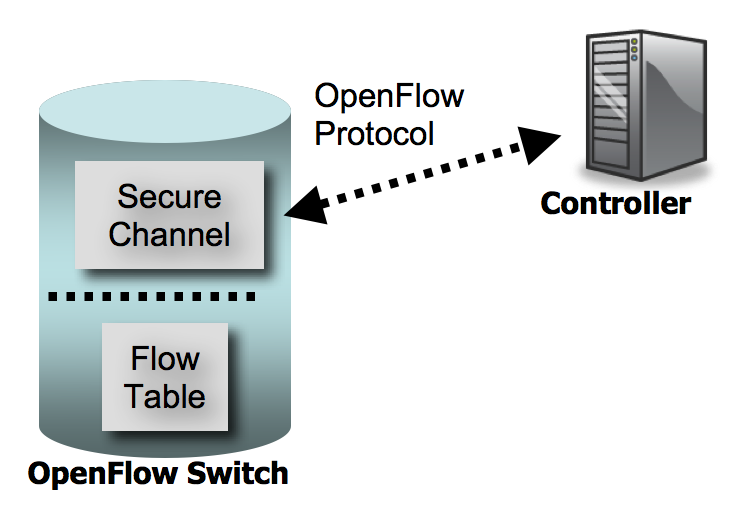
\includegraphics[height=2.5in]{figure_flow_table_secchan.png}
\caption{An OpenFlow switch communicates with a controller over a secure connection using the OpenFlow protocol.}
\label{fig:flow table and controller}
\end{figure}

\section{Switch Components}
An OpenFlow Switch consists of a \emph{flow table}, which performs packet lookup and forwarding, and a \emph{secure channel} to an external controller (Figure \ref{fig:flow table and controller}).  The controller manages the switch over the secure channel using the OpenFlow protocol.
\\\\
The flow table contains a set of flow entries (header values to match packets against), activity counters, and a set of zero or more actions to apply to matching packets.  All packets processed by the switch are compared against the flow table.  If a matching entry is found, any actions for that entry are performed on the packet (e.g., the action might be to forward a packet out a specified port).  If no match is found, the packet is forwarded to the controller over the secure channel.  The controller is responsible for determining how to handle packets without valid flow entries, and it manages the switch flow table by adding and removing flow entries.
\\\\
Flow entries may forward packets to one or more OpenFlow ports.   In general, these are physical ports, but the protocol does not preclude abstractions like port aggregations or VLAN traffic on a port appearing as an OpenFlow port.  OpenFlow ports have limited state such as ``up'', ``down'' and whether spanning tree flood packets should be forwarded out the port.  Additional configuration of ports may handled by the OpenFlow configuration protocol.  There are several OpenFlow virtual ports used to indicate, for example, flooding or the ingress port (see \ref{ft:actions}).

\section{Flow Table}
This section describes the components of flow table entries and the process by which incoming packets are matched against flow table entries.  

\begin{table}[hbp]
\centering
\begin{tabular}{|c|c|c|}
\hline	
Header Fields & Counters & Actions\\ 
\hline	
\end{tabular}
\caption{A flow entry consists of header fields, counters, and actions.}
\label{table:flow entry}
\end{table}

Each flow table entry (see Table \ref{table:flow entry}) contains: 
\begin{itemize} 
\item \textbf{header fields} to match against packets 
\item \textbf{counters} to update for matching packet 
\item \textbf{actions} to apply to matching packets 
\end{itemize} 

\subsection{Header Fields}
\begin{table}[hbp]
\centering
\footnotesize
\begin{tabularx}{\textwidth}{ |X|X|X|X|X|X|X|X|X|X|X|X| }
\hline
Ingress Port &
Ether source &
Ether dst &
Ether type &
VLAN id &
VLAN priority &
IP src &
IP dst &
IP proto &
IP ToS bits &
TCP/ UDP src port &
TCP/ UDP dst port
\\ 
\hline
\end{tabularx}
\caption{Fields from packets used to match against flow entries.}
\label{table:header fields}
\end{table}

Table \ref{table:header fields} shows the header fields an incoming packet is compared against. Each entry contains a specific value, or ANY, which matches any value. If the switch supports subnet masks on the IP source and/or destination fields, these can more precisely specify matches.  The fields in the OpenFlow 12-tuple are listed in Table \ref{table:header fields} and details on the properties of each field are described in Table \ref{table:header field details}.
\\\\
\begin{table}[hbp]
\centering
\footnotesize
\begin{tabularx}{\textwidth}{ |X|X|X|X| }
\hline Field & Bits & When applicable & Notes \\
\hline Ingress Port & (Implementation dependent) & All packets & Numerical representation of incoming port, starting at 1.  \\
\hline Ethernet source address & 48 & All packets on enabled ports & \\
\hline Ethernet destination address & 48 & All packets on enabled ports & \\ 
\hline Ethernet type & 16 & All packets on enabled ports & An OpenFlow switch is required to match the type in both standard Ethernet and 802.2 with a SNAP header and OUI of 0x000000.  The special value of 0x05FF is used to match all 802.3 packets without SNAP headers. \\
\hline VLAN id & 12 & All packets of Ethernet type 0x8100 & \\
\hline VLAN priority & 3 & All packets of Ethernet type 0x8100 & VLAN PCP field \\
\hline IP source address & 32 & All IP and ARP packets & Can be subnet masked \\
\hline IP destination address & 32 & All IP and ARP packets & Can be subnet masked \\
\hline IP protocol & 8 & All IP and IP over Ethernet, ARP packets & Only the lower 8 bits of the ARP opcode are used \\
\hline IP ToS bits & 6 & All IP packets & Specify as 8-bit value and place ToS in upper 6 bits. \\
\hline Transport source port / ICMP Type & 16 & All TCP, UDP, and ICMP packets & Only lower 8 bits used for ICMP Type \\
\hline Transport destination port / ICMP Code & 16 & All TCP, UDP, and ICMP packets & Only lower 8 bits used for ICMP Code \\
\hline
\end{tabularx}
\caption{Field lengths and the way they must be applied to flow entries.}
\label{table:header field details}
\end{table}Switch designers are free to implement the internals in any way convenient provided that correct functionality is preserved.  For example, while a flow may have multiple forward actions, each specifying a different port, a switch designer may choose to implement this as a single bitmask within the hardware forwarding table.

\subsection{Counters}

Counters are maintained per-table, per-flow, \qosupd{per-port and
  per queue}.  OpenFlow-compliant counters may be implemented in software and maintained by polling hardware counters with more limited ranges.
\\\\
Table \ref{table:counters} contains the required set of counters.  Duration refers to the time the flow has been installed in the switch.  The Receive Errors field includes all explicitly specified errors, including frame, overrun, and CRC errors, plus any others.  Counters wrap around with no overflow indicator.  In this document, the phrase byte refers to 8-bit octets.
\begin{table}[!hbp] 	
\centering
\footnotesize
%\begin{tabularx}{\textwidth}{ |X|X| }
\begin{tabular}{ |l|c| }
\hline Counter & Bits	 \\
\hline \multicolumn{2}{|c|}{Per Table} \\
\hline Active Entries & 32 \\
\hline Packet Lookups & 64 \\
\hline Packet Matches & 64 \\
\hline \multicolumn{2}{|c|}{Per Flow} \\
\hline Received Packets & 64 \\
\hline Received Bytes & 64 \\
\hline Duration (seconds) & 32 \\
\hline Duration (nanoseconds) & 32 \\
\hline  \multicolumn{2}{|c|}{Per Port} \\
\hline Received Packets & 64 \\
\hline Transmitted Packets & 64 \\
\hline Received Bytes & 64 \\
\hline Transmitted Bytes & 64 \\
\hline Receive Drops & 64 \\
\hline Transmit Drops & 64 \\
\hline Receive Errors & 64 \\
\hline Transmit Errors & 64 \\
\hline Receive Frame Alignment Errors & 64 \\
\hline Receive Overrun Errors & 64 \\
\hline Receive CRC Errors & 64 \\
\hline Collisions & 64 \\
\hline  \multicolumn{2}{|c|}{\qosupd{Per Queue}} \\
\hline \qosupd{Transmit Packets} & \qosupd{64} \\
\hline \qosupd{Transmit Bytes} & \qosupd{64} \\
\hline \qosupd{Transmit Overrun Errors} & \qosupd{64}\\
\hline
\end{tabular}
\caption{Required list of counters for use in statistics messages.}
\label{table:counters}
\end{table}

\subsection{Actions}
\label{ft:actions}
Each flow entry is associated with zero or more actions that dictate how the switch handles matching packets.  If no forward actions are present, the packet is dropped.  Action lists for \emph{inserted} flow entries MUST be processed in the order specified.  However, there is no packet output ordering guaranteed within a port.   For example, an action list may result in two packets sent to two different VLANs on a single port.  These two packets may be arbitrarily re-ordered, but the packet bodies must match those generated from a sequential execution of the actions.
\\\\
A switch may reject a flow entry if it cannot process the action list in the order specified, in which case it should immediately return an unsupported flow error (see \ref{unsupported_flow}).  Ordering within a port may vary between vendor switch implementations.
\\\\
A switch is not required to support all action types --- just those marked ``Required Actions'' below. When connecting to the controller, a switch indicates which of the ``Optional Actions'' it supports.  OpenFlow-compliant switches come in two types: \emph{OpenFlow-only}, and \emph{OpenFlow-enabled}. 
\\\\
OpenFlow-only switches support only the required actions below, while OpenFlow-enabled switches, routers, and access points may also support the \textbf{NORMAL} action.  Either type of switch can also support the \textbf{FLOOD} action.
\\\\
\textbf{Required Action:} \textit{Forward}. 
OpenFlow switches must support forwarding the packet to physical ports and the following virtual ones:
\begin{itemize}
\item \textbf{ALL:} Send the packet out all interfaces, not including the incoming interface.
\item \textbf{CONTROLLER:} Encapsulate and send the packet to the controller.
\item \textbf{LOCAL:} Send the packet to the switch�s local networking stack.
\item \textbf{TABLE:} Perform actions in flow table.  Only for packet-out messages.
\item \textbf{IN\_PORT:} Send the packet out the input port. 
\end{itemize}
\textbf{Optional Action:} \textit{Forward}.
The switch may optionally support the following virtual ports:
\begin{itemize}
\item \textbf{NORMAL:} Process the packet using the traditional forwarding path supported by the switch (i.e., traditional L2, VLAN, and L3 processing.)  The switch may check the VLAN field to determine whether or not to forward the packet along the normal processing route.  If the switch cannot forward entries for the OpenFlow-specific VLAN back to the normal processing route, it must indicate that it does not support this action.
\item \textbf{FLOOD:} Flood the packet along the minimum spanning tree, not including the incoming interface.
\end{itemize}
The controller will only ask the switch to send to multiple physical ports simultaneously if the switch indicates it supports this behavior in the initial handshake (see section \ref{cts:handshake}).  
\\\\
\textbf{\qosupd{Optional Action:}} \emph{\qosupd{Enqueue}}. \qosupd{The enqueue action forwards
a packet through a queue attached to a port. Forwarding behavior is
dictated by the configuration of the queue and is used to provide
basic Quality-of-Service (QoS) support (see section \ref{cts:qos}).}
\\\\
\textbf{Required Action:} \emph{Drop}.  A flow-entry with no specified action indicates that all matching packets should be dropped.
\\\\
\textbf{Optional Action:} \emph{Modify-Field}.  While not strictly required, the actions shown in Table \ref{table:field modify actions}  greatly increase the usefulness of an OpenFlow implementation.  To aid integration with existing networks, we suggest that VLAN modification actions be supported. 

\begin{table}[hbp]
\centering
\footnotesize
\begin{tabularx}{\linewidth}{ |X|X|X| }
\hline
Action & Associated Data & Description \\
\hline
Set VLAN ID &
12 bits &
If no VLAN is present, a new header is added with the specified VLAN ID and priority of zero.

If a VLAN header already exists, the VLAN ID is replaced with the specified value. \\
\hline
Set VLAN priority &
3 bits &
If no VLAN is present, a new header is added with the specified priority and a VLAN ID of zero.  

If a VLAN header already exists, the priority field is replaced with the specified value. \\
\hline
Strip VLAN header &
- &
Strip VLAN header if present. \\
\hline
Modify Ethernet source MAC address &
48 bits: Value with which to replace existing source MAC address &
Replace the existing Ethernet source MAC address with the new value \\
\hline
Modify Ethernet destination MAC address &
48 bits: Value with which to replace existing destination MAC address &
Replace the existing Ethernet destination MAC address with the new value. \\
\hline
Modify IPv4 source address & 
32 bits: Value with which to replace existing IPv4 source address &
Replace the existing IP source address with new value and update the IP checksum (and TCP/UDP 
checksum if applicable). 

This action is only applicable to IPv4 packets. \\
\hline
Modify IPv4 destination address & 
32 bits: Value with which to replace existing IPv4 destination address &
Replace the existing IP destination address with new value and update the IP checksum (and TCP/UDP checksum if applicable).

This action is only applied to IPv4 packets. \\
\hline
Modify IPv4 ToS bits &
6 bits: Value with which to replace existing IPv4 ToS field &
Replace the existing IP ToS field.
This action is only applied to IPv4 packets. \\
\hline
Modify transport source port &
16 bits: Value with which to replace existing TCP or UDP source port &
Replace the existing TCP/UDP source port with new value and update the TCP/UDP checksum.

This action is only applicable to TCP and UDP packets.\\
\hline
Modify transport destination port & 
16 bits: Value with which to replace existing TCP or UDP destination port &
Replace the existing TCP/UDP destination port with new value and update the TCP/UDP checksum

This action is only applied to TCP and UDP packets.\\
\hline
\end{tabularx}
\caption{Field-modify actions.}
\label{table:field modify actions}
\end{table}

\subsection{Matching}
\begin{figure}[!htb]
\centering
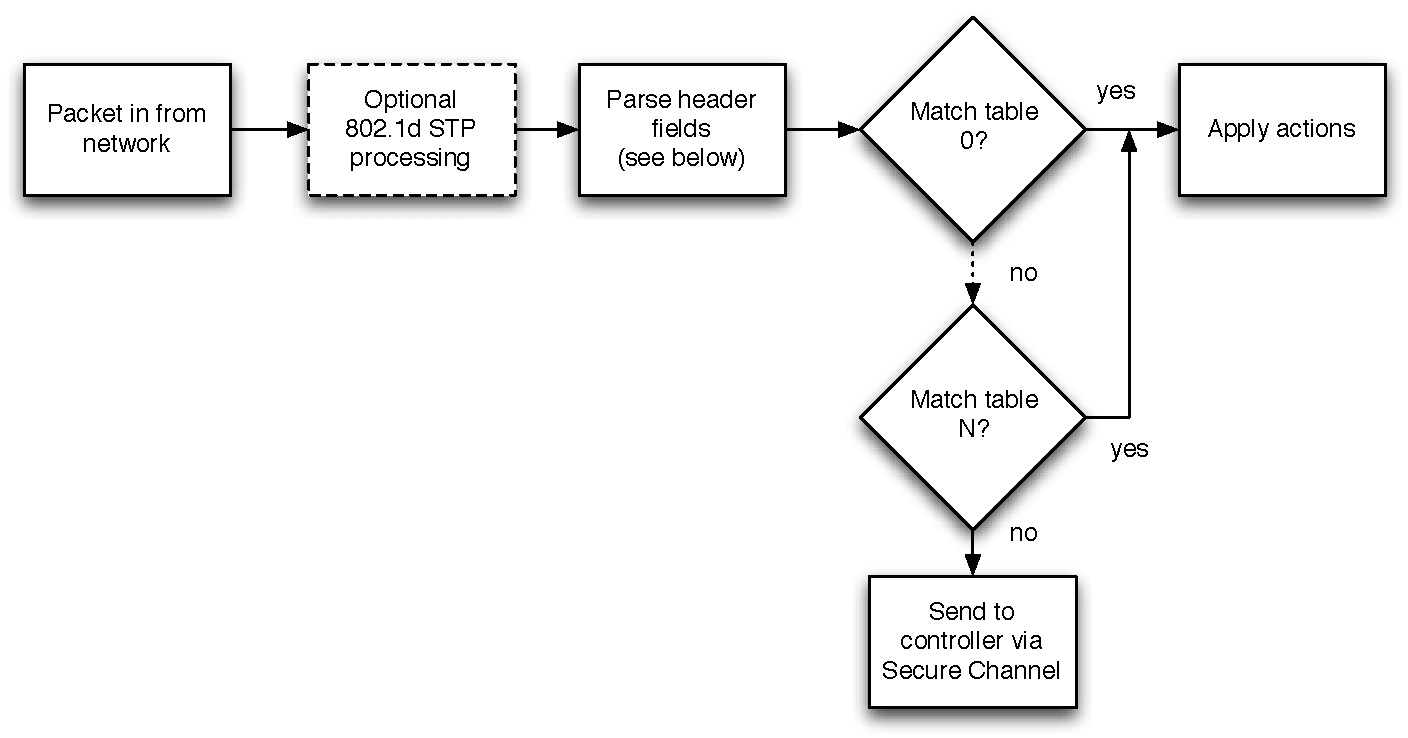
\includegraphics[height=1.85in]{packet_flow_flowchart}
\caption{Packet flow in an OpenFlow switch.  As discussed in Section \ref{flow_table:stp_support}, support for 802.1D is optional.}
\label{fig:packet_flow}
\end{figure}

\begin{figure}[!htb]
\centering
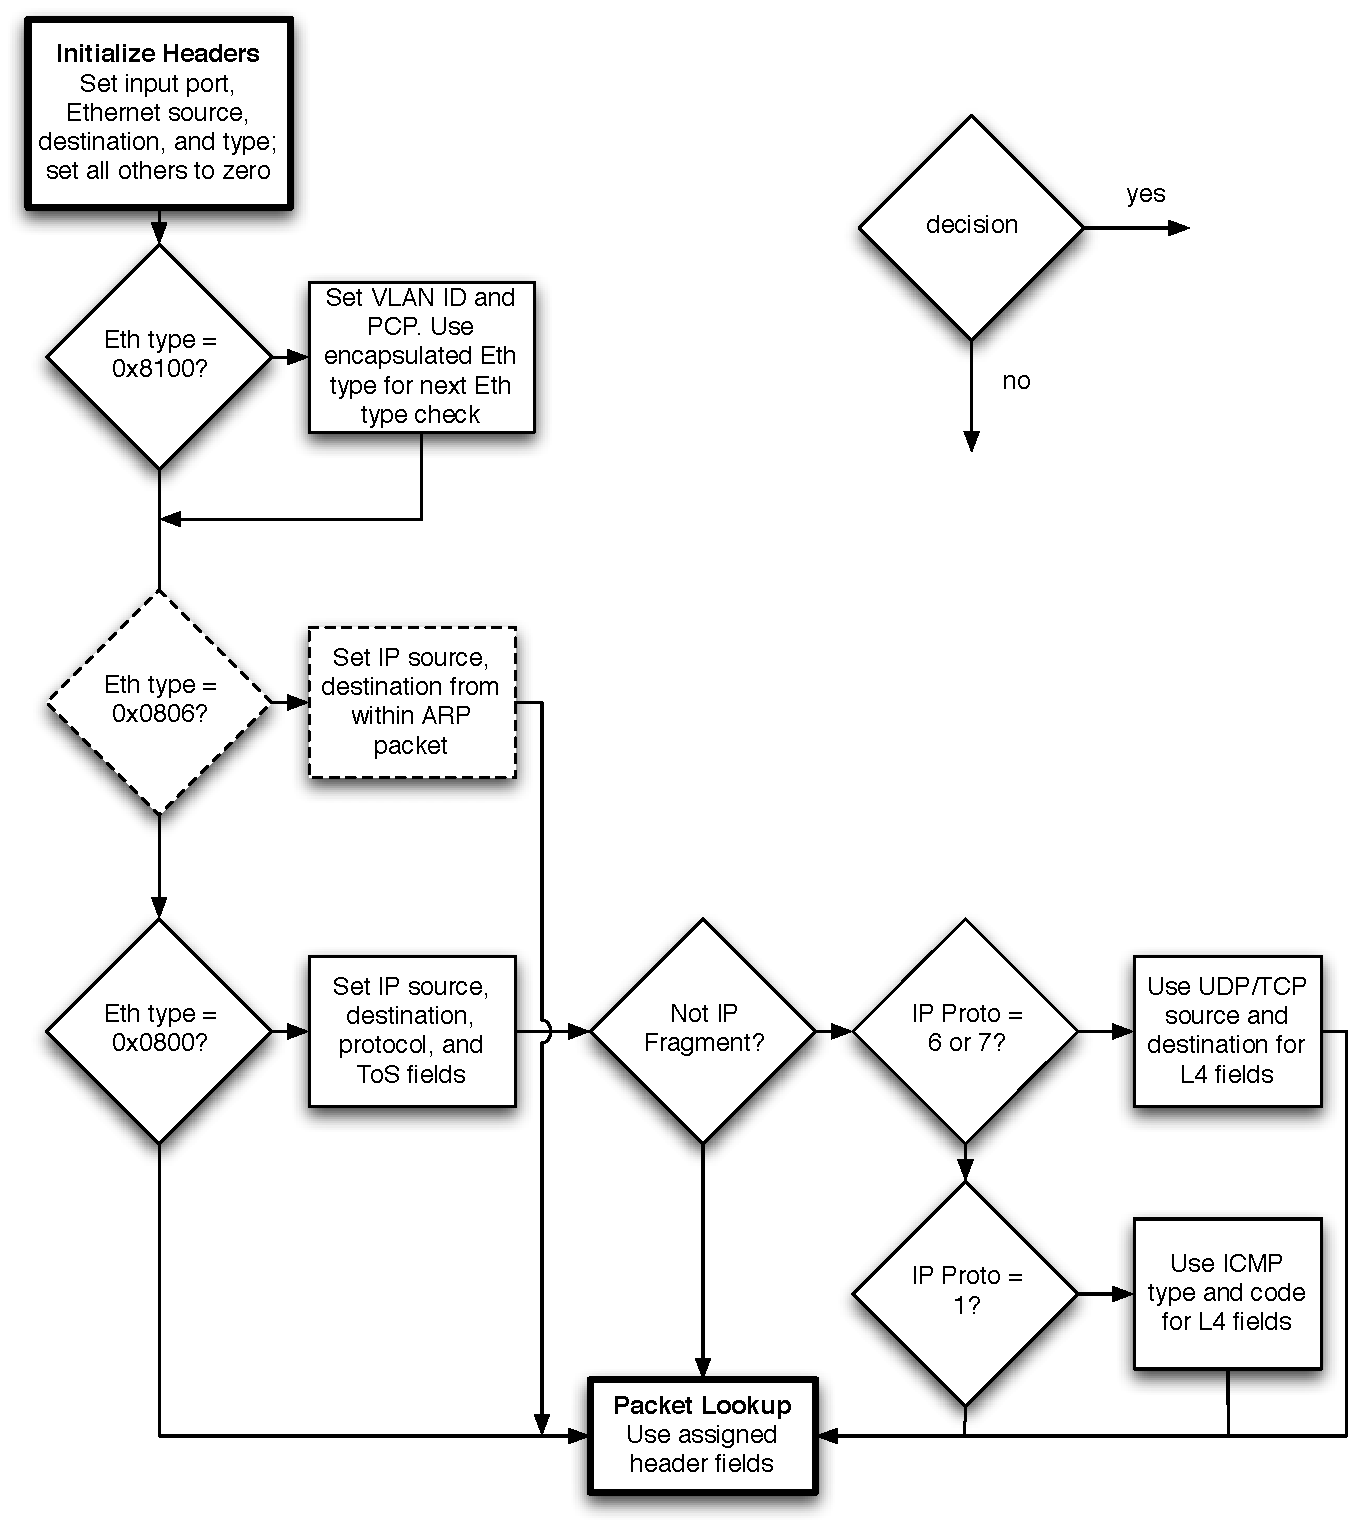
\includegraphics[height=2.9in]{header_parsing_flowchart}
\caption{Flowchart showing how header fields are parsed for matching.}
\label{fig:header_parsing}
\end{figure}

On receipt of a packet, an OpenFlow Switch performs the functions shown in Figure \ref{fig:packet_flow}.  Header fields used for the table lookup depend on the packet type as described below (and shown in Figure \ref{fig:header_parsing}).

\begin{itemize}
\item Rules specifying an ingress port are matched against the physical port that received the packet.
\item The Ethernet headers as specified in Table \ref{table:header fields} are used for all packets.
\item If the packet is a VLAN (Ethernet type 0x8100), the VLAN ID and PCP fields are used in the lookup.
\item (Optional) For ARP packets (Ethernet type equal to 0x0806), the lookup fields may also include the contained IP source and destination fields.
\item For IP packets (Ethernet type equal to 0x0800), the lookup fields also include those in the IP header.
\item For IP packets that are TCP or UDP (IP protocol is equal to 6 or 17), the lookup includes the transport ports.
\item For IP packets that are ICMP (IP prototcol is equal to 1), the lookup includes the Type and Code fields.  
\item For IP packets with nonzero fragment offset or More Fragments bit set, the transport ports are set to zero for the lookup.
\end{itemize}
A packet matches a flow table entry if the values in the header fields used for the lookup (as defined above) match those defined in the flow table.  If a flow table field has a value of ANY, it matches all possible values in the header.  
\\\\
To handle the various Ethernet framing types, matching the Ethernet type is handled in a slightly different manner.  If the packet is an Ethernet II frame, the Ethernet type is handled in the expected way.  If the packet is an 802.3 frame with a SNAP header and Organizationally Unique Identifier (OUI) of 0x000000, the SNAP protocol id is matched against the flow�s Ethernet type.  A flow entry that specifies an Ethernet type of 0x05FF, matches all Ethernet 802.2 frames without a SNAP header and those with SNAP headers that do not have an OUI of 0x000000.  
\\\\
Packets are matched against flow entries based on prioritization.  An entry that specifies an exact match (i.e., it has no wildcards) is always the highest priority.  All wildcard entries have a priority associated with them.  Higher priority entries must match before lower priority ones.  If multiple entries have the same priority, the switch is free to choose any ordering.  Higher numbers have higher priorities.
\\\\
For each packet that matches a flow entry, the associated counters for that entry are updated.  If no matching entry can be found for a packet, the packet is sent to the controller over the secure channel.

\section{Secure Channel}
The secure channel is the interface that connects each OpenFlow switch to a controller.  Through this interface, the controller configures and manages the switch, receives events from the switch, and send packets out the switch.
\\\\
Between the datapath and the secure channel, the interface is implementation-specific, however all secure channel messages must be formatted according to the OpenFlow protocol. 
\\\\
Support for multiple simultaneous controllers is currently undefined.

\subsection{OpenFlow Protocol Overview}
The OpenFlow protocol supports three message types, \emph{controller-to-switch}, \emph{asynchronous}, and \emph{symmetric}, each with multiple sub-types.  Controller-to-switch messages are initiated by the controller and used to directly manage or inspect the state of the switch.  Asynchronous messages are initiated by the switch and used to update the controller of network events and changes to the switch state. Symmetric messages are initiated by either the switch or the controller and sent without solicitation.  The message types used by OpenFlow are described below.

\subsubsection{Controller-to-Switch}
Controller/switch messages are initiated by the controller and may or may not require a response from the switch.
\\\\
\textbf{Features:}  Upon Transport Layer Security (TLS) session establishment, the controller sends a features request message to the switch.  The switch must reply with a features reply that specifies the capabilities supported by the switch.
\\\\
\textbf{Configuration:} The controller is able to set and query configuration parameters in the switch.  The switch only responds to a query from the controller.
\\\\
\textbf{Modify-State:} Modify-State messages are sent by the controller to manage state on the switches.  Their primary purpose is to add/delete and modify flows in the flow tables and to set switch port properties.  
\\\\
\textbf{Read-State:} Read-State messages are used by the controller to collect statistics from the switch�s flow-tables, ports and the individual flow entries.
\\\\\
\textbf{Send-Packet}:  These are used by the controller to send packets out of a specified port on the switch.
\\\\
\textbf{Barrier}: Barrier request/reply messages are used by the controller to ensure message dependencies have been met or to receive notifications for completed operations.  

\subsubsection{Asynchronous}
Asynchronous messages are sent without the controller soliciting them from a switch.  Switches send asynchronous messages to the controller to denote a packet arrival, switch state change, or error.  The four main asynchronous message types are described below.
\\\\
\textbf{Packet-in:} For all packets that do not have a matching flow entry, a packet-in event is sent to the controller (or if a packet matches an entry with a ``send to controller" action).  If the switch has sufficient memory to buffer packets that are sent to the controller, the packet-in events contain some fraction of the packet header (by default \input{define/OFP_DEFAULT_MISS_SEND_LEN} bytes) and a buffer ID to be used by the controller when it is ready for the switch to forward the packet.  Switches that do not support internal buffering (or have run out of internal buffering) must send the full packet to the controller as part of the event.
\\\\
\textbf{Flow-Removed:} When a flow entry is added to the switch by a flow modify message, an idle timeout value indicates when the entry should be removed due to a lack of activity, as well as a hard timeout value that indicates when the entry should be removed, regardless of activity.  The flow modify message also specifies whether the switch should send a flow removed message to the controller when the flow expires.  Flow modify messages which delete flows may also cause flow removed messages.
\\\\
\textbf{Port-status:} The switch is expected to send port-status messages to the controller as port configuration state changes.  These events include change in port status (for example, if it was brought down directly by a user) or a change in port status as specified by 802.1D (see Section \ref{flow_table:stp_support} for a description of 802.1D support requirements).
\\\\
\textbf{Error:} The switch is able to notify the controller of problems using error messages. 

\subsubsection{Symmetric}
Symmetric messages are sent without solicitation, in either direction.
\\\\
\textbf{Hello:} Hello messages are exchanged between the switch and controller upon connection startup.
\\\\
\textbf{Echo:} Echo request/reply messages can be sent from either the switch or the controller, and must return an echo reply.  They can be used to indicate the latency, bandwidth, and/or liveness of a controller-switch connection.
\\\\
\textbf{Vendor:} Vendor messages provide a standard way for OpenFlow switches to offer additional functionality within the OpenFlow message type space.  This is a staging area for features meant for future OpenFlow revisions.

\subsection{Connection Setup}
The switch must be able to establish the communication at a user-configurable (but otherwise fixed) IP address, using a user-specified port.  Traffic to and from the secure channel is not checked against the flow table.  Therefore, the switch must identify incoming traffic as local before checking it against the flow table.  Future versions of the protocol specification will describe a dynamic controller discovery protocol in which the IP address and port for communicating with the controller is determined at runtime.
\\\\
When an OpenFlow connection is first established, each side of the connection must immediately send an \verb|OFPT_HELLO| message with the \verb|version| field set to the highest OpenFlow protocol version supported by the sender.  Upon receipt of this message, the recipient may calculate the OpenFlow protocol version to be used as the smaller of the version number that it sent and the one that it received.
\\\\
If the negotiated version is supported by the recipient, then the connection proceeds. Otherwise, the recipient must reply with an \verb|OFPT_ERROR| message with a \verb|type| field of \verb|OFPET_HELLO_FAILED|, a \verb|code| field of \verb| OFPHFC_COMPATIBLE|, and optionally an ASCII string explaining the situation in \verb|data|, and then terminate the connection.

\subsection{Connection Interruption}
In the case that a switch loses contact with the controller, as a result of a echo request timeout, TLS session timeout, or other disconnection, it should attempt to contact one or more backup controllers.  The ordering of the controller IP addresses is not specified by the protocol.
\\\\
If some number of attempts to contact a controller (zero or more) fail, the switch must enter ``emergency mode'' and immediately reset the current TCP connection.  In emergency mode, the matching process is dictated by the emergency flow table entries (those marked with the emergency bit when added to the switch).  All normal entries are deleted when entering emergency mode.
\\\\
Upon connecting to a controller again, the emergency flow entries remain.  The controller then has the option of deleting all flow entries, if desired.
\\\\
The first time a switch starts up, it is considered to be in emergency mode.  Configuration of the default set of flow entries is outside the scope of the OpenFlow protocol.

\subsection{Encryption}
The switch and controller communicate through a TLS connection.  The TLS connection is initiated by the switch on startup to the controller's server, which is located by default on TCP port \input{define/OFP_TCP_PORT}.   The switch and controller mutually authenticate by exchanging certificates signed by a site-specific private key.  Each switch must be user-configurable with one certificate for authenticating the controller (controller certificate) and the other for authenticating to the controller (switch certificate).

\subsection{Spanning Tree}
\label{flow_table:stp_support}
OpenFlow switches may optionally support 802.1D Spanning Tree Protocol.  Those switches that do support it are expected to process all 802.1D packets locally before performing flow lookup.  A switch that implements STP must set the \verb|OFPC_STP| bit in the 'capabilities' field of its \verb|OFPT_FEATURES_REPLY| message. A switch that implements STP must make it available on all of its physical ports, but it need not implement it on virtual ports (e.g. \verb|OFPP_LOCAL|). 
\\\\
Port status, as specified by the spanning tree protocol, is then used to limit packets forwarded to the \verb|OFP_FLOOD| port to only those ports along the spanning tree.  Port changes as a result of the spanning tree are sent to the controller via port-update messages.  Note that forward actions that specify the outgoing port or \verb|OFP_ALL| ignore the port status set by the spanning tree protocol.  Packets received on ports that are disabled by spanning tree must follow the normal flow table processing path. 
\\\\
Switches that do not support 802.1D spanning tree must allow the controller to specify the port status for packet flooding through the port-mod messages. 

\subsection{Flow Table Modification Messages}
\label{flow_table:sec_chan:flow_add}
\label{flow_table:sec_chan:flow_mod}
\label{flow_table:sec_chan:flow_removal}
Flow table modification messages can have the following types:
\input{enum/ofp_flow_mod_command}
For ADD requests with the \verb|OFPFF_CHECK_OVERLAP| flag set, the switch must first check for any overlapping flow entries.  Two flow entries overlap if a single packet may match both, and both entries have the same priority.  If an overlap conflict exists between an existing flow entry and the ADD request, the switch must refuse the addition and respond with an \verb|ofp_error_msg| with \verb|OFPET_FLOW_MOD_FAILED| type and \verb|OFPFMFC_OVERLAP| code.
\\\\
For valid (non-overlapping) ADD requests, or those with no overlap checking, the switch must insert the flow entry at the lowest numbered table for which the switch supports all wildcards set in the \verb|flow_match| struct, and for which the priority would be observed during the matching process.  If a flow entry with identical header fields and priority already resides in any table, then that entry, including its counters, must be removed, and the new flow entry added.
\\\\
If a switch cannot find any table in which to add the incoming flow entry, the switch should send an \verb|ofp_error_msg| with \verb|OFPET_FLOW_MOD_FAILED| type and \verb|OFPFMFC_ALL_TABLES_FULL| code.
\\\\
If the action list in a flow mod message references a port that will never be valid on a switch, the switch must return an \verb|ofp_error_msg| with \verb|OFPET_BAD_ACTION| type and \verb|OFPBAC_BAD_OUT_PORT| code.  If the referenced port may be valid in the future, e.g. when a linecard is added to a chassis switch, or a port is dynamically added to a software switch, the switch may either silently drop packets sent to the referenced port, or immediately return an \verb|OFPBAC_BAD_OUT_PORT| error and refuse the flow mod.
\\\\
For MODIFY requests, if a flow entry with identical header fields does not current reside in any table, the MODIFY acts like an ADD, and the new flow entry must be inserted with zeroed counters.  Otherwise, the actions field is changed on the existing entry and its counters and idle time fields are left unchanged.
\\\\
For DELETE requests, if no flow entry matches, no error is recorded, and no flow table modification occurs.  If flow entries match, and must be deleted, then each normal entry with the \verb|OFPFF_SEND_FLOW_REM| flag set should generate a flow removed message.  Deleted emergency flow entries generate no flow removed messages.
\\\\
MODIFY and DELETE flow mod commands have corresponding \_STRICT versions.   Without \_STRICT appended, the wildcards are active and all flows that match the description are modified or removed.  If \_STRICT is appended, all fields, including the wildcards and priority, are strictly matched against the entry, and only an identical flow is modified or removed.  For example, if a message to remove entries is sent that has all the wildcard flags set, the DELETE command would delete all flows from all tables, while the DELETE\_STRICT command would only delete a rule that applies to all packets at the specified priority.
\\\\
For non-strict MODIFY and DELETE commands that contain wildcards, a match will occur when a flow entry exactly matches or is more specific than the description in the flow\_mod command. For example, if a DELETE command says to delete all flows with a destination port of 80, then a flow entry that is all wildcards will not be deleted. However, a DELETE command that is all wildcards will delete an entry that matches all port 80 traffic.  This same interpretation of mixed wildcard and exact header fields also applies to individual and aggregate flows stats.  
\\\\
DELETE and DELETE\_STRICT commands can be optionally filtered by output port.  If the \verb|out_port| field contains a value other than \verb|OFPP_NONE|, it introduces a constraint when matching.  This constraint is that the rule must contain an output action directed at that port.  This field is ignored by ADD, MODIFY, and MODIFY\_STRICT messages.
\\\\
Emergency flow mod messages must have timeout values set to zero.  Otherwise, the switch must refuse the addition and respond with an \verb|ofp_error_msg| with \verb|OFPET_FLOW_MOD_FAILED| type and \verb|OFPFMFC_BAD_EMERG_TIMEOUT| code.
\\\\
\label{unsupported_flow}If a switch cannot process the action list for any flow mod message in the order specified, it MUST immediately return an \verb|OFPET_FLOW_MOD_FAILED| :
\verb|OFPFMFC_UNSUPPORTED| error and reject the flow.

\subsection{Flow Removal}

Each flow entry has an \verb|idle_timeout| and a \verb|hard_timeout| associated with it.  If no packet has matched the rule in the last \verb|idle_timeout| seconds, or it has been \verb|hard_timeout| seconds since the flow was inserted, the switch removes the entry and sends a flow removed message.  In addition, the controller is able to actively remove entries by sending a flow message with the \verb|DELETE| or \verb|DELETE_STRICT| command.  Like the message used to add the entry, a removal message contains a description, which may include wild cards.

%\appendix
\section{Appendix A: The OpenFlow Protocol}
The heart of the OpenFlow spec is the set of structures used for OpenFlow Protocol messages.  
\\\\
The structures, defines, and enumerations described below are derived from the file \verb|include/openflow/openflow.h|, which is part of the standard OpenFlow distribution.  All structures are packed with padding and 8-byte aligned, as checked by the assertion statements.  All OpenFlow messages are sent in big-endian format.  

\subsection{OpenFlow Header}
Each OpenFlow message begins with the OpenFlow header:

\input{struct/ofp_header}
The version specifies the OpenFlow protocol version being used.  During the current draft phase of the OpenFlow Protocol, the most significant bit will be set to indicate an experimental version and the lower bits will indicate a revision number.  The current version is \input{define/OFP_VERSION}.  The final version for a Type 0 switch will be 0x00.  The length field indicates the total length of the message, so no additional framing is used to distinguish one frame from the next.  The type can have the following values:

\input{enum/ofp_type}

\subsection{Common Structures}
This section describes structures used by multiple messages.

\subsubsection{Port Structures}
Physical ports are described with the following structure:

\input{struct/ofp_phy_port}
The \verb|port_no| field is a value the datapath associates with a physical port.  The \verb|hw_addr| field typically is the MAC address for the port; \verb|OFP_MAX_ETH_ALEN| is 6.  The name field is a null-terminated string containing a human-readable name for the interface.  The value of \verb|OFP_MAX_PORT_NAME_LEN| is 16.  
\\\\
The \verb|config| field describes spanning tree and administrative settings with the following structure:

\input{enum/ofp_port_config}
The port config bits indicate whether a port has been administratively brought down, options for handling 802.1D spanning tree packets, and how to handle incoming and outgoing packets.   These bits, configured over multiple switches, enable an OpenFlow network to safely flood packets along either a custom or 802.1D spanning tree.
\\\\
The controller may set \verb|OFPPFL_NO_STP| to 0 to enable STP on a port or to 1 to disable STP on a port. (The latter corresponds to the Disabled STP port state.) The default is switch implementation-defined; the OpenFlow reference implementation by default sets this bit to 0 (enabling STP).
\\\\
When \verb|OFPPFL_NO_STP| is 0, STP controls the \verb|OFPPFL_NO_FLOOD| and \verb|OFPPFL_STP_*| bits directly. \verb|OFPPFL_NO_FLOOD| is set to 0 when the STP port state is Forwarding, otherwise to 1. The bits in \verb|OFPPFL_STP_MASK| are set to one of the other \verb|OFPPFL_STP_*| values according to the current STP port state.
\\\\
When the port flags are changed by STP, the switch sends an \verb|OFPT_PORT_STATUS| message to notify the controller of the change. The \verb|OFPPFL_NO_RECV|, \verb|OFPPFL_NO_RECV_STP|, \verb|OFPPFL_NO_FWD|, and \verb|OFPPFL_NO_PACKET_IN| bits in the OpenFlow port flags may be useful for the controller to implement STP, although they interact poorly with in-band control. 
\\\\
The \verb|state| field describes the spanning tree state and whether a physical link is present, with the following structure:

\input{enum/ofp_port_state}
All port state bits are read-only, representing spanning tree and physical link state.
\\\\
The port numbers use the following conventions:

\input{enum/ofp_port}
The \verb|curr|, \verb|advertised|, \verb|supported|, and \verb|peer| fields indicate link modes (10M to 10G full and half-duplex), link type (copper/fiber) and link features (autonegotiation and pause).  Port features are represent by the following structure:

\input{enum/ofp_port_features}
Multiple of these flags may be set simultaneously.

\subsubsection{Flow Match Structures}
When describing a flow entry, the following structure is used:

\input{struct/ofp_match}
The \verb|wildcards| field has a number of flags that may be set:

\input{enum/ofp_flow_wildcards}
If no wildcards are set, then the \verb|ofp_match| exactly describes a flow, over the entire OpenFlow 11-tuple.  On the other extreme, if all the wildcard flags are set, then every flow will match.  
\\\\
The source and destination netmasks are each specified with a 6-bit number in the wildcard description. It is interpreted similar to the CIDR suffix, but with the opposite meaning, since this is being used to indicate which bits in the IP address should be treated as ``wild". For example, a CIDR suffix of "24" means to use a netmask of ``255.255.255.0". However, a wildcard mask value of ``24" means that the least-significant 24-bits are wild, so it forms a netmask of ``255.0.0.0". 

\subsubsection{Flow Action Structures}
A number of actions may be associated with flows or packets.  The currently defined action types are:

\input{enum/ofp_action_type} 
Output actions are described in Section \ref{ft:actions}, while Field-Modify actions are described in Table \ref{table:field modify actions}.  An action definition contains the action type, length, and any associated data:

\input{struct/ofp_action_header}
An \verb|action_output| has the following fields:

\input{struct/ofp_action_output}
The \verb|max_len| indicates the maximum amount of data from a packet that should be sent when the port is \verb|OFPP_CONTROLLER|.  If \verb|max_len| is zero, the switch must send a zero-size \verb|packet_in| message.  The \verb|port| specifies the physical port from which packets should be sent. 
 \\\\
An \verb|action_vlan_vid| has the following fields:

\input{struct/ofp_action_vlan_vid}
The \verb|vlan_vid| field is 16 bits long, when an actual VLAN id is only 12 bits. The value \verb|0xffff| is used to indicate that no VLAN id was set.
\\\\
An \verb|action_vlan_pcp| has the following fields:

\input{struct/ofp_action_vlan_pcp}
The \verb|vlan_pcp| field is 8 bits long, but only the lower 3 bits have meaning.  
\\\\
An \verb|action_strip_vlan| takes no arguments and consists only of a generic \verb|ofp_action_header|.  This action strips the VLAN tag if one is present.
\\\\
An \verb|action_dl_addr| has the following fields:

\input{struct/ofp_action_dl_addr}
The \verb|dl_addr| field is the MAC address to set.
\\\\
An \verb|action_nw_addr| has the following fields:

\input{struct/ofp_action_nw_addr}
The \verb|nw_addr| field is the IP address to set.
\\\\
An \verb|action_nw_tos| has the following fields:

\input{struct/ofp_action_nw_tos}
The \verb|nw_tos| field is the 6 upper bits of the ToS field to set, in the original bit positions (shifted to the left by 2).
\\\\
An \verb|action_tp_port| has the following fields:

\input{struct/ofp_action_tp_port}
The \verb|tp_port| field is the TCP/UDP/other port to set.
\\\\
An \verb|action_vendor| has the following fields:

\input{struct/ofp_action_vendor_header}
The \verb|vendor| field is the Vendor ID, which takes the same form as in struct \verb|ofp_vendor|.

\subsection{Controller-to-Switch Messages}

\subsubsection{Handshake}
\label{cts:handshake} 
Upon SSL session establishment, the controller sends an \verb|OFPT_FEATURES_REQUEST| message.  This message does not contain a body beyond the OpenFlow header.  The switch responds with an \verb|OFPT_FEATURES_REPLY| message:

\input{struct/ofp_switch_features}
The \verb|datapath_id| field uniquely identifies a datapath.  The lower 48 bits are intended for the switch MAC address, while the top 16 bits are up to the implementer.  An example use of the top 16 bits would be a VLAN ID to distinguish multiple virtual switch instances on a single physical switch.  This field should be treated as an opaque bit string by controllers.
\\\\
The \verb|n_tables| field describes the number of tables supported by the switch, each of which can have a different set of supported wildcard bits and number of entries.  When the controller and switch first communicate, the controller will find out how many tables the switch supports from the Features Reply. If it wishes to understand the size, types, and order in which tables are consulted, the controller sends a \verb|OFPST_TABLE| stats request. A switch must return these tables in the order the packets traverse the tables, with all exact-match tables listed before all tables with wildcards.
\\\\
The \verb|capabilities| field uses the following flags:

\input{enum/ofp_capabilities} 
The \verb|actions| field is a bitmap of supported actions on the hardware.  It uses the values from \verb|ofp_action_type| as the number of bits to shift left for an associated action.  For example, \verb|OFPAT_SET_DL_VLAN| would use the flag \verb|0x00000002|.
\\\\
The \verb|ports| field is an array of \verb|ofp_phy_port| structures that describe all the physical ports in the system that support OpenFlow.  The number of port elements is inferred from the length field in the OpenFlow header. 

\subsubsection{Switch Configuration}
The controller is able to set and query configuration parameters in the switch with the \verb|OFPT_SET_CONFIG| and \verb|OFPT_GET_CONFIG_REQUEST| messages, respectively.  The switch responds to a configuration request with an \verb|OFPT_GET_CONFIG_REPLY| message; it does not reply to a request to set the configuration.  
\\\\
There is no body for \verb|OFPT_GET_CONFIG_REQUEST| beyond the OpenFlow header.  The \verb|OFPT_SET_CONFIG| and \verb|OFPT_GET_CONFIG_REPLY| use the following:

\input{struct/ofp_switch_config}
The configuration flags include the following:

\input{enum/ofp_config_flags}
The \verb|OFPC_FRAG_*| flags indicate whether IP fragments should be treated normally, dropped, or reassembled.  ``Normal" handling of fragments means that an attempt should be made to pass the fragments through the OpenFlow tables. If any field is not present (e.g., the TCP/UDP ports didn't fit), then the packet should not match any entry that has that field set.
\\\\
The \verb|miss_send_len| field defines the number of bytes of each packet sent to the controller as a result of both flow table misses and flow table hits with the controller as the destination.  If this field equals 0, the switch must send a zero-size \verb|packet_in| message.

\subsubsection{Modify State Messages}
\paragraph{Modify Flow Entry Message}
Modifications to the flow table from the controller are done with the \verb|OFPT_FLOW_MOD| message:

\input{struct/ofp_flow_mod}
The \verb|command| field must be one of the following:

\input{enum/ofp_flow_mod_command}
The differences between \verb|OFPFC_MODIFY| and \verb|OFPFC_MODIFY_STRICT| are explained in Section \ref{flow_table:sec_chan:flow_mod} and differences between \verb|OFPFC_DELETE| and \verb|OFPFC_DELETE_STRICT| are explained in Section \ref{flow_table:sec_chan:flow_removal}. 
\\\\
The \verb|idle_timeout| and \verb|hard_timeout| fields control how quickly flows expire.  
\\\\
If the \verb|idle_timeout| is set and the \verb|hard_timeout| is zero, the entry must expire after \verb|idle_timeout| seconds with no received traffic.  If the \verb|idle_timeout| is zero and the \verb|hard_timeout| is set, the entry must expire in \verb|hard_timeout| seconds regardless of whether or not packets are hitting the entry.
\\\\
If both \verb|idle_timeout| and \verb|hard_timeout| are set, the flow will timeout after \verb|idle_timeout| seconds with no traffic, or \verb|hard_timeout| seconds, whichever comes first.  If both \verb|idle_timeout| and \verb|hard_timeout| are zero, the entry is considered permanent and will never time out.  It can still be removed with a \verb|flow_mod| message of type \verb|OFPFC_DELETE|. 
\\\\
The \verb|priority| field is only relevant for flow entries with wildcard fields.  The priority field indicates table priority, where higher numbers are higher priorities; the switch must keep the highest-priority wildcard entries in the lowest-numbered (fastest) wildcard table, to ensure correctness.  It is the responsibility of each switch implementer to ensure that exact entries always match before wildcards entries, regardless of the table configuration.  
\\\\
The \verb|buffer_id| refers to a buffered packet sent by the \verb|OFPT_PACKET_IN| message.
\\\\
The \verb|out_port| field optionally filters the scope of DELETE and DELETE\_STRICT messages by output port.  If \verb|out_port| contains a value other than \verb|OFPP_NONE|, it introduces a constraint when matching.  This constraint is that the rule must contain an output action directed at that port.  Other constraints such as \verb|ofp_match| structs and priorities are still used; this is purely an \emph{additional} constraint.  Note that to disable output port filtering, \verb|out_port| must be set to \verb|OFPP_NONE|, since 0 is a valid port id.  This field is ignored by ADD, MODIFY, and MODIFY\_STRICT messages.
\\\\
The \verb|flags| field may include the follow flags:

\input{enum/ofp_flow_mod_flags}
When the \verb|OFPFF_SEND_FLOW_REM| flag is set, the switch must send a flow removed message when the flow expires.  The default is for the switch to not send flow removed messages for newly added flows.  
\\\\
When the \verb|OFPFF_CHECK_OVERLAP| flag is set, the switch must check that there are no conflicting entries with the same priority. If there is one, the flow mod fails and an error code is returned.
\\\\
When the \verb|OFPFF_EMERG_| flag is set, the switch must consider this flow entry as an emergency entry, and only use it for forwarding when disconnected from the controller.

\paragraph{Port Modification Message}
The controller uses the \verb|OFPT_PORT_MOD| message to modify the behavior of the physical port:

\input{struct/ofp_port_mod}
The \verb|mask| field is used to select bits in the \verb|config| field to change.  The \verb|advertise| field has no mask; all port features change together.

\subsubsection{Read State Messages}
While the system is running, the datapath may be queried about its current state using the \verb|OFPT_STATS_REQUEST| message:

\input{struct/ofp_stats_request}
The switch responds with one or more \verb|OFPT_STATS_REPLY| messages:

\input{struct/ofp_stats_reply}
The only value defined for \verb|flags| in a reply is whether more replies will follow this one - this has the value \verb|0x0001|.  To ease implementation, the switch is allowed to send replies with no additional entries.  However, it must always send another reply following a message with the �more� flag set.  The transaction ids (xid) of replies must always match the request that prompted them.
\\\\
In both the request and response, the \verb|type| field specifies the kind of information being passed and determines how the \verb|body| field is interpreted:

\input{enum/ofp_stats_types}

\paragraph{Description Statistics}
Information about the switch manufacturer, hardware revision, software revision, serial number, and a description field is available from the \verb|OFPST_DESC| stats request type:

\input{struct/ofp_desc_stats}
Each entry is ASCII formatted and padded on the right with 0 bytes.  \verb|DESC_STR_LEN| is \input{define/DESC_STR_LEN}and \verb|SERIAL_NUM_LEN| is \input{define/SERIAL_NUM_LEN}.  Note: \footnote{Added to address concerns raised in  \url{https://mailman.stanford.edu/pipermail/openflow-spec/2009-September/000504.html}} the dp\_desc field is a free-form string to describe the datapath for debugging purposes, e.g., ``switch3 in room 3120''.  As such, it is not guaranteed to be unique and should not be used as the primary identifier for the datapath---use the datapath\_id field from the switch features instead (\S~\ref{cts:handshake}).

\paragraph{Individual Flow Statistics}
Information about individual flows is requested with the \verb|OFPST_FLOW| stats request type:

\input{struct/ofp_flow_stats_request}
The \verb|match| field contains a description of the flows that should be matched and may contain wildcards.  This field's matching behavior is described in Section \ref{flow_table:sec_chan:flow_add}.
\\\\
The \verb|table_id| field indicates the index of a single table to read, or \verb|0xff| for all tables.
\\\\
The \verb|out_port| field optionally filters by output port.  If \verb|out_port| contains a value other than \verb|OFPP_NONE|, it introduces a constraint when matching.  This constraint is that the rule must contain an output action directed at that port.  Other constraints such as \verb|ofp_match| structs are still used; this is purely an \emph{additional} constraint.  Note that to disable output port filtering, \verb|out_port| must be set to \verb|OFPP_NONE|, since 0 is a valid port id. 
\\\\
The \verb|body| of the reply consists of an array of the following:

\input{struct/ofp_flow_stats}
The fields consist of those provided in the \verb|flow_mod| that created these, plus the table into which the entry was inserted, the packet count, and the byte count.
\\\\
\label{flow_duration_info}The \verb|duration_sec| and \verb|duration_nsec| fields indicate the elapsed time the flow has been installed in the switch. The total duration in nanoseconds can be computed as $\verb|duration_sec|*10^{9}$ + \verb|duration_nsec|. Implementations are required to provide millisecond precision; higher precision is encouraged where available.

\paragraph{Aggregate Flow Statistics}
Aggregate information about multiple flows is requested with the \verb|OFPST_AGGREGATE| stats request type:

\input{struct/ofp_aggregate_stats_request}
The \verb|match| field contains a description of the flows that should be matched and may contain wildcards.  This field's matching behavior is described in Section \ref{flow_table:sec_chan:flow_add}.
\\\\
The \verb|table_id| field indicates the index of a single table to read, or \verb|0xff| for all tables.
\\\\
The \verb|out_port| field optionally filters by output port.  If \verb|out_port| contains a value other than \verb|OFPP_NONE|, it introduces a constraint when matching.  This constraint is that the rule must contain an output action directed at that port.  Other constraints such as \verb|ofp_match| structs are still used; this is purely an \emph{additional} constraint.  Note that to disable output port filtering, \verb|out_port| must be set to \verb|OFPP_NONE|, since 0 is a valid port id. 
\\\\
The \verb|body| of the reply consists of the following:

\input{struct/ofp_aggregate_stats_reply} 

\paragraph{Table Statistics}
Information about tables is requested with the \verb|OFPST_TABLE| stats request type.  The request does not contain any data in the body.
\\\\
The body of the reply consists of an array of the following:

\input{struct/ofp_table_stats}
The \verb|body| contains a \verb|wildcards| field, which indicates the fields for which that particular table supports wildcarding. For example, a direct look-up hash table would have that field set to zero, while a sequentially searched table would have it set to \verb|OFPFW_ALL|. The entries are returned in the order that packets traverse the tables. 
\\\\
\verb|OFP_MAX_TABLE_NAME_LEN| is \input{define/OFP_MAX_TABLE_NAME_LEN}.

\paragraph{Port Statistics}
Information about physical ports is requested with the \verb|OFPST_PORT| stats request type.  The request does not contain any data in the \verb|body|.
\\\\
The body of the reply consists of an array of the following:

\input{struct/ofp_port_stats}
The switch should return a value of -1 for unavailable counters.

\paragraph{Vendor Statistics}
Vendor-specific stats messages are requested with the \verb|OFPST_VENDOR| stats type. The first four bytes of the message are the vendor identifier. The rest of the body is vendor-defined.
\\\\
The \verb|vendor| field is a 32-bit value that uniquely identifies the vendor. If the most significant byte is zero, the next three bytes are the vendor's IEEE OUI. If vendor does not have (or wish to use) their OUI, they should contact the OpenFlow consortium to obtain one. 

\subsubsection{Send Packet Message}
When the controller wishes to send a packet out through the datapath, it uses the \verb|OFPT_PACKET_OUT| message:

\input{struct/ofp_packet_out}
The \verb|buffer_id| is the same given in the \verb|ofp_packet_in| message.  If the \verb|buffer_id| is -1, then the packet data is included in the data array. If \verb|OFPP_TABLE| is specified as the output port of an action, the \verb|in_port| in the \verb|packet_out| message is used in the flow table lookup.

\subsubsection{Barrier Message}
When the controller wants to ensure message dependencies have been met or wants to receive notifications for completed operations, it may use an \verb|OFPT_BARRIER_REQUEST| message.  This message has no body.  Upon receipt, the switch must finish processing all previously-received messages before executing any messages beyond the Barrier Request.  When such processing is complete, the switch must send an \verb|OFPT_BARRIER_REPLY| message with the \verb|xid| of the original request.

\subsection{Asynchronous Messages}
\subsubsection{Packet-In Message}
When packets are received by the datapath and sent to the controller, they use the \verb|OFPT_PACKET_IN| message:

\input{struct/ofp_packet_in}
The \verb|buffer_id| is an opaque value used by the datapath to identify a buffered packet.  When a packet is buffered, some number of bytes from the message will be included in the data portion of the message.  If the packet is sent because of a ``send to controller'' action, then \verb|max_len| bytes from the \verb|action_output| of the flow setup request are sent.  If the packet is sent because of a flow table miss, then at least \verb|miss_send_len| bytes from the \verb|OFPT_SET_CONFIG| message are sent.  The default \verb|miss_send_len| is \input{define/OFP_DEFAULT_MISS_SEND_LEN}bytes.  If the packet is not buffered, the entire packet is included in the data portion, and the \verb|buffer_id| is -1.  
\\\\
Switches that implement buffering are expected to expose, through documentation, both the amount of available buffering, and the length of time before buffers may be reused.  A switch must gracefully handle the case where a buffered \verb|packet_in| message yields no response from the controller.  A switch should prevent a buffer from being reused until it has been handled by the controller, or some amount of time (indicated in documentation) has passed.
\\\\
The reason field can be any of these values:

\input{enum/ofp_packet_in_reason}
 
\subsubsection{Flow Removed Message}
If the controller has requested to be notified when flows time out, the datapath does this with the \verb|OFPT_FLOW_REMOVED| message:

\input{struct/ofp_flow_removed}
The \verb|match| and \verb|priority| fields are the same as those used in the flow setup request.  
\\\\
The \verb|reason| field is one of the following:

\input{enum/ofp_flow_removed_reason}
The \verb|duration_sec| and \verb|duration_nsec| fields are described in Section \ref{flow_duration_info}.
\\\\
The \verb|idle_timeout| field is directly copied from the flow mod that created this entry. 
\\\\
With the above three fields, one can find both the amount of time the flow was active, as well as the amount of time the flow received traffic.
\\\\
The \verb|packet_count| and \verb|byte_count| indicate the number of packets and bytes that were associated with this flow, respectively. 
 
\subsubsection{Port Status Message}
As physical ports are added, modified, and removed from the datapath, the controller needs to be informed with the \verb|OFPT_PORT_STATUS| message:

\input{struct/ofp_port_status}
The \verb|status| can be one of the following values:

\input{enum/ofp_port_reason} 

\subsubsection{Error Message}
There are times that the switch needs to notify the controller of a problem.  This is done with the \verb|OFPT_ERROR_MSG| message: 	

\input{struct/ofp_error_msg}
The \verb|type| value indicates the high-level type of error.  The \verb|code| value is interpreted based on the type.  The \verb|data| is variable length and interpreted based on the \verb|type| and \verb|code|; in most cases this is the message that caused the problem.  
\\\\
Error codes ending in \verb|_EPERM| correspond to a permissions error generated by an entity between a controller and switch, such as an OpenFlow hypervisor. 
\\\\
Currently defined error types are:

\input{enum/ofp_error_type}
For the \verb|OFPET_HELLO_FAILED| error \verb|type|, the following \verb|code|s are currently defined:

\input{enum/ofp_hello_failed_code}
The \verb|data| field contains an ASCII text string that adds detail on why the error occurred.
\\\\
For the \verb|OFPET_BAD_REQUEST| error \verb|type|, the following \verb|code|s are currently defined:

\input{enum/ofp_bad_request_code}
The \verb|data| field contains at least 64 bytes of the failed request.
\\\\
For the \verb|OFPET_BAD_ACTION| error \verb|type|, the following \verb|code|s are currently defined:

\input{enum/ofp_bad_action_code}
The \verb|data| field contains at least 64 bytes of the failed request.
\\\\
For the \verb|OFPET_FLOW_MOD_FAILED| error \verb|type|, the following \verb|code|s are currently defined:

\input{enum/ofp_flow_mod_failed_code}
The \verb|data| field contains at least 64 bytes of the failed request.
\\\\
If the error message is in response to a specific message from the controller, e.g., \verb|OFPET_BAD_REQUEST|, \verb|OFPET_BAD_ACTION|, or \verb|OFPET_FLOW_MOD_FAILED|, then the \verb|xid| field of the header should match that of the offending message.

\subsection{Symmetric Messages}
\subsubsection{Hello}
The \verb|OFPT_HELLO| message has no body; that is, it consists only of an OpenFlow header. Implementations must be prepared to receive a hello message that includes a body, ignoring its contents, to allow for later extensions. 

\subsubsection{Echo Request}
An Echo Request message consists of an OpenFlow header plus an arbitrary-length data field.  The data field might be a message timestamp to check latency, various lengths to measure bandwidth, or zero-size to verify liveness between the switch and controller.

\subsubsection{Echo Reply}
An Echo Reply message consists of an OpenFlow header plus the unmodified data field of an echo request message.
\\\\
In an OpenFlow protocol implementation divided into multiple layers, the echo request/reply logic should be implemented in the "deepest" practical layer.  For example, in the OpenFlow reference implementation that includes a userspace process that relays to a kernel module, echo request/reply is implemented in the kernel module.  Receiving a correctly formatted echo reply then shows a greater likelihood of correct end-to-end functionality than if the echo request/reply were implemented in the userspace process, as well as providing more accurate end-to-end latency timing.

\subsubsection{Vendor}
The Vendor message is defined as follows:

\input{struct/ofp_vendor_header}
The \verb|vendor| field is a 32-bit value that uniquely identifies the vendor. If the most significant byte is zero, the next three bytes are the vendor's IEEE OUI. If vendor does not have (or wish to use) their OUI, they should contact the OpenFlow consortium to obtain one. The rest of the body is uninterpreted.
\\\\
If a switch does not understand a vendor extension, it must send an \verb|OFPT_ERROR| message with a \verb|OFPBRC_BAD_VENDOR| error code and \verb|OFPET_BAD_REQUEST| error type. 



\section{Appendix B: Credits}

Current Maintainer: Brandon Heller (brandonh@stanford.edu).
\\\\
Spec contributions, in alphabetical order:
\\\\
Ben Pfaff,
Brandon Heller,
Dan Talayco,
David Erickson,
Glen Gibb,
Guido Appenzeller,
Jean Tourrilhes,
Justin Pettit,
KK Yap,
Martin Casado,
Masayoshi Kobayashi,
Nick McKeown,
Peter Balland,
Reid Price,
Rob Sherwood,
Yiannis Yiakoumis.
 
\end{document} 
